\documentclass[11pt,reqno]{amsart}
\usepackage{tikz}
\usepackage{tikz-cd}
\usepackage{amssymb}
\usepackage{hyperref,xcolor}
\usetikzlibrary{arrows.meta, positioning}

\begin{document}

    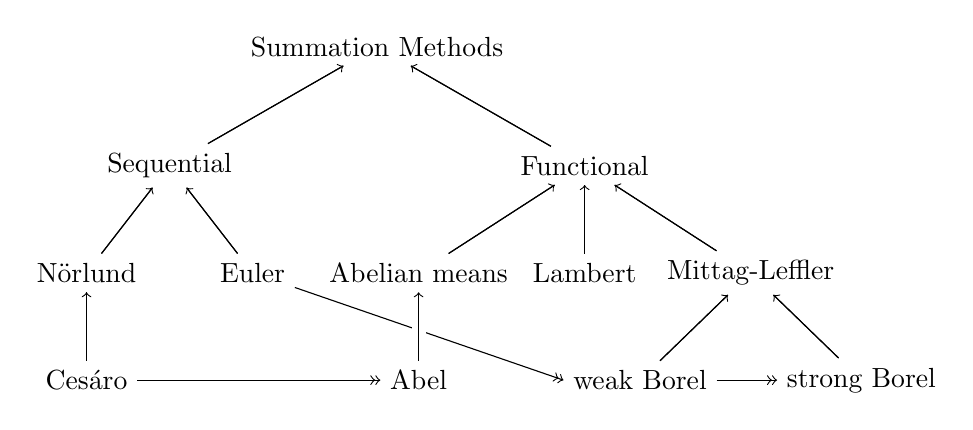
\begin{tikzpicture}[on top/.style={preaction={draw=white,-,line width=#1}},
on top/.default=4pt, >={Classical TikZ Rightarrow[]}]
        \node (SM) {Summation Methods}[sibling distance = 15em, level distance = 10ex]
            child {node (S) {Sequential} [sibling distance = 6em, level distance = 9ex]
            child {node (N) {N\"{o}rlund} [sibling distance = 6em, level distance = 9ex]
            child {node (C) {Ces\'{a}ro}}}
            child {node (E) {Euler}}}
            child {node (F) {Functional} [sibling distance = 6em, level distance = 9ex]
            child {node (AM) {Abelian means} [sibling distance = 6em, level distance = 9ex]
            child {node (A) {Abel}}}
            child {node (L) {Lambert}}
            child {node (M) {Mittag-Leffler}
            [sibling distance = 8em, level distance = 9ex] child {node (WB) {weak Borel}}
            child {node (SB) {strong Borel}}}};
        \draw [->>] (C) -- (A);
        \draw [->>] (WB) -- (SB);
        \draw [->>] (E) -- (WB.west);
        \draw [<-] (N) -- (C);
        \draw [<-, on top = 5pt] (AM) -- (A);
        \draw [<-] (M) -- (WB);
        \draw [<-] (M) -- (SB);
        \draw [<-] (SM) -- (S);
        \draw [<-] (SM) -- (F);
        \draw [<-] (S) -- (N);
        \draw [<-] (S) -- (E);
        \draw [<-] (F) -- (AM);
        \draw [<-] (F) -- (L);
        \draw [<-] (F) -- (M);
    \end{tikzpicture}

\end{document}